组帧只需要掌握四种方法,分别是\textbf{:字符计数法、字节填充的首尾界符法、比特填充的首尾标志法、违规编码违例法。}

\textbf{{1. 字符计数法}}\\

字符计数法是\textbf{{用一个特殊的字符来表示一帧的开始,然后用一个计数字段来表明该帧包含的字节数}}。当目的主机接收到该帧时,根据此字段提供的字节数,便可知道该帧的结束位和下一帧的开始位,如图3-2所示。

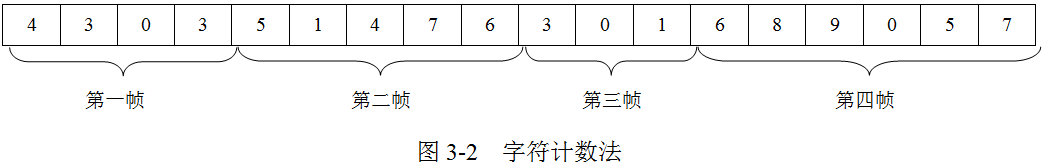
\includegraphics[width=6in]{png-jpeg-pics/33417908A56A9F2D821F07E23FBD244B.png}

\textbf{{2. 字节填充的首尾界符法}}

由C语言的知识可以知道ASCII码是7位编码,可以组成128个不同的ASCII码,但是可以打印(就是可以从键盘输入的字符)的只有95个字符,那么当传送的帧是文本文件(都是从键盘输入的)时,就可以在剩下的33个控制字符中选定2个字符(教材中选用了SOH与EOT分别作为帧开始符和帧结束符)作为每一帧的开始和结束,这样接收端只需要判断这两个控制字符出现的位置就能准确地分割成帧,如图3-3所示。

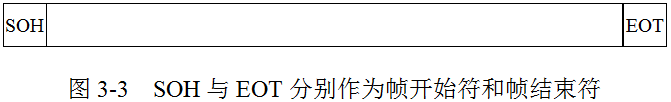
\includegraphics[width=6in]{png-jpeg-pics/1DA8665C7083D19C0B49D679D4A326FD.png}

这种方式对于帧数据为文本文件是绝对没有问题的。但是还有一种情况就比较麻烦了,假设要传送的帧不是文本文件,即帧数据部分可能包含控制字符,就不能仅仅使用控制字符去进行帧定界了,否则将会导致错误地``找到帧的边界'',把部分帧收下(误认为是一个完整的帧),如图3-4所示。\\
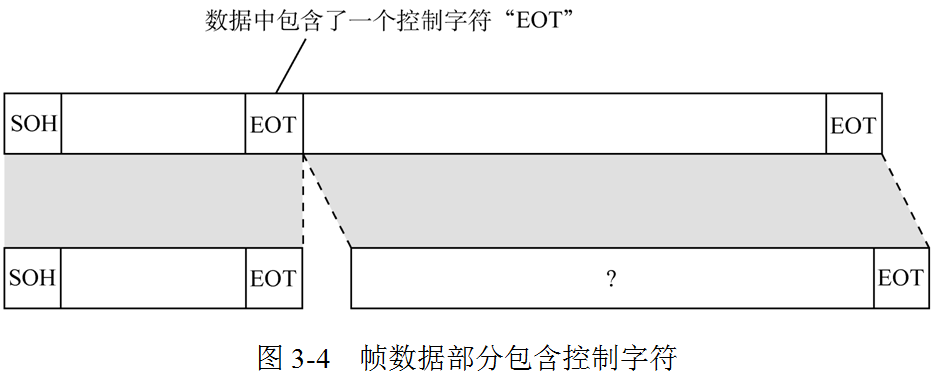
\includegraphics[width=6in]{png-jpeg-pics/A2D71F83E75A76E0EC484845517030F7.png}

从图3-3中可以看出确实解决了帧定界问题,但是从图3-4中看得出并不是所有比特流都可以被正确地传输,所以说此时透明传输问题仍未得到解决,首尾界符法是不严谨的,于是出现了字节填充的首尾界符法。\\
字节填充的首尾界符法设法将数据中可能出现的控制字符``SOH''{和``EOT''在接收端不解释为控制字符。}

\textbf{其方法如下:}

在数据中出现字符``SOH''或``EOT''时就将其转换为另一个字符,而这个字符是不会被错误解释的。但所有字符都有可能在数据中出现,于是就将数据中出现的字符``SOH''转换为``ESC''和``x''两个字符,将数据中出现的字符``EOT''转换为``ESC''和``y''两个字符。而当数据中出现了控制字符``ESC''时,就将其转换为``ESC''和``z''两个字符。这种转换方法能够在接收端将收到的数据正确地还原为原来的数据。``ESC''是转义符,它的十六进制编码是1B。\\
如图3-5所示,在上方的数据中出现了4个控制字符``ESC''、``EOT''、``ESC''和``SOH''。按以上规则转换后的数据即为图3-5下方的数据。

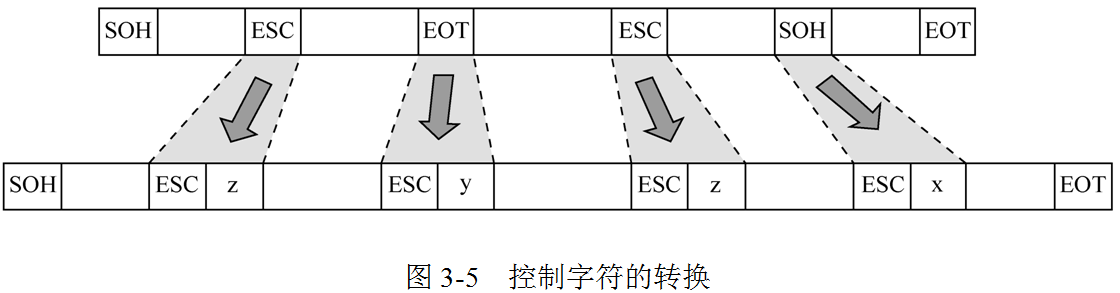
\includegraphics[width=3.33333in,height=0.87500in]{png-jpeg-pics/47B60388BAD2BCBCFD0ACE2224A9BF28.png}

读者可以很容易地看出,在接收端只要按照以上转换规则进行相反的转换,就能够还原出原来的数据(如遇到``ESC''和``z'',就还原为``ESC'')。

\textbf{{3. 比特填充的首尾标志法}}

比特填充的首尾标志法是{\textbf{使用01111110作为帧的开始和结束标志}},似乎帧定界又解决了,但是如果帧数据部分出现了01111110怎么办?透明传输仍然是个问题。\textbf{其解决方法如下:}\\
不难发现01111110中有6个连续的``1'',只要数据帧检测到有5个连续的``1'',马上在其后插入``0'',而接收方做该过程的逆操作,即每收到5个连续的``1'',自动删除后面紧跟的``0'',以恢复原始数据。因此,此方法又称为零比特填充法,具体可见下面的模拟过程。

\textbf{模拟过程:}\\
1)原始数据。0110101111110010111111011(数据中出现两次01111110)。\\
2)零比特填充后的数据。011010111110100101111101011(加下画线的0表示填充的0)。\\
3)接收方收到数据,一旦遇到5个连续的``1''就将后面的``0''去掉,即可得到原始数据。

\textbf{{4. 物理编码违例法}}

物理编码违例法利用物理介质上编码的违法标志来区分帧的开始与结束,例如,在曼彻斯特编码中,码元1编码成高-低电平,码元0编码成低-高电平,而高-高和低-低电平的编码方式是无效的,可以分别用来作为帧的起始标志和结束标志。
